\chapter{CirMetrics: Công cụ phân tích và quản lí mạch ZKP}
\label{chap:chap6}
\section{Giới thiệu}
CirMetrics là một ứng dụng hỗ trợ phát triển mạch ZKP, được nghiên cứu xây dựng từ nhu cầu thực tế trong việc tối ưu hóa hiệu suất biên dịch và tạo bằng chứng. Xuất phát từ nghiên cứu về chiến lược tối ưu hóa trong sử dụng trình biên dịch Circom, CirMetrics được phát triển nhằm mang lại một quy trình đánh giá hiệu quả, chính xác và trực quan hơn cho các nhà phát triển ZKP.

Ứng dụng này giúp người dùng theo dõi các thông số quan trọng trong quá trình biên dịch và tạo bằng chứng, bao gồm số lượng constraint theo từng loại, thời gian biên dịch và thời gian tạo proof. Tất cả được hiển thị bằng biểu đồ trực quan, giúp nhà phát triển dễ dàng nhận diện các vấn đề về hiệu năng và xu hướng thay đổi trong quá trình phát triển mạch.

Điểm đặc biệt của CirMetrics chính là khả năng mở rộng, hướng tới việc tích hợp các gợi ý tối ưu hóa tự động dựa trên giai đoạn phát triển của dự án. Điều này giúp các nhà phát triển Circom lựa chọn chiến lược biên dịch phù hợp, giảm chi phí tạo bằng chứng và tối ưu hóa quy trình từ nguyên mẫu đến sản phẩm hoàn chỉnh.
\section{Phân tích thiết kế}
Công cụ CirMetrics được thiết kế để phục vụ trực tiếp cho các nhà phát triển ứng dụng ZKP. Công cụ này được thiết kế để đáp ứng những mục tiêu như sau:

\begin{itemize}
    \item Giúp những nhà phát triển ứng dụng sử dụng ZKP có thể quản lí và theo dõi các thông số của mạch trong quá trình phát triển ứng dụng:
    \begin{itemize}
        \item Hiển thị thống kê ràng buộc: Số lượng ràng buộc tuyến tính, phi tuyến tính, tổng số ràng buộc.
        \item Theo dõi thời gian biên dịch: Đo lường thời gian biên dịch với các cờ tối ưu hóa khác nhau.
        \item Quản lí thời gian tạo bằng chứng: Người dùng có thể theo dõi và quản lí thời gian tạo bằng chứng sau mỗi lần chỉnh sửa và áp dụng các mức tối ưu ràng buộc khác nhau.
    \end{itemize}
    \item Trực quan hoá dữ liệu: Hỗ trợ hiển thị và so sánh các thông số mạch tương ứng với các mức tối ưu hóa khác nhau. Bên cạnh đó công cụ cũng hỗ trợ trực quan hoá tần suất cập nhật mạch cũng như tần suất tạo bằng chứng thông qua các biểu đồ, giúp các nhà phát triển thuận tiện hơn khi lựa chọn phương pháp tối ưu mạch trong quá trình phát triển dự án.
\end{itemize}

Bảng \ref{tab:use_case_cirmetrics} dưới đây mô tả các chức năng của CirMetrics:

\begin{table}[h]
    \centering
    \begin{tabular}{|l|p{7cm}|}
        \hline
        \textbf{Chức Năng} & \textbf{Mô Tả} \\ \hline
        Thực hiện phân tích mạch & Cho phép người viết mạch upload mạch, thực hiện biên dịch mạch và tạo bằng chứng trên giao diện công cụ CirMetrics\\ \hline
        Xem các kết quả phân tích & Hiển thị thống số của các mạch đã biên dịch và tạo bằng chứng theo thời gian. \\ \hline
        Xem tổng hợp các biểu đồ & So sánh và trực quan hóa các thông số liên quan đến mạch ZK và quá trình phát triển mạch.
        \\ \hline
    \end{tabular}
    \caption{Bảng Use Case cho công cụ CirMetrics}
    \label{tab:use_case_cirmetrics}
\end{table}
\section{Kiến trúc hệ thống}

CirMetrics được thiết kế theo kiến trúc Client-Server nhằm phân chia nhiệm vụ riêng biệt cho các thành phần khác nhau, giúp tối ưu hóa hiệu suất và quản lý tài nguyên tập trung. Nó cho phép mở rộng hệ thống dễ dàng và bảo vệ dữ liệu tốt hơn trên server. Kiến trúc ứng dụng này gồm các lớp sau:
\begin{itemize}
    \item Lớp giao diện (Front-end): Ứng dụng sử dụng ReactJS kết hợp với thư viện shadcn/ui để hỗ trợ thiết kế giao diện. Mục tiêu là giúp CirMetrics mang đến trải nghiệm trực quan và dễ sử dụng, giúp người dùng theo dõi và tương tác với dữ liệu một cách thuận tiện.
    \item Lớp xử lí nghiệp vụ (Back-end): Phần backend của CirMetrics được phát triển bằng Javascripts với NodeJS. Thành phần này chịu trách nhiệm tiếp nhận và xử lý các yêu cầu từ phía giao diện, thực hiện phân tích dữ liệu biên dịch, lưu trữ thông tin cần thiết và cung cấp API phục vụ cho giao diện.
    \item Lớp cơ sở dữ liệu (Database): Dữ liệu hệ thống được lưu trữ bằng SQLite, phù hợp với tính chất nhẹ, đơn giản và dễ triển khai cho ứng dụng hỗ trợ trong quá trình phát triển. Cơ sở dữ liệu này lưu trữ thông tin về các phiên biên dịch, số lượng constraint, thời gian thực thi và các dữ liệu phân tích liên quan.
\end{itemize}
\begin{figure}[H]
    \centering
    
\includegraphics[width=\textwidth]{imgs/ToolsApp.png}
    \caption{Kiến trúc hệ thống CirMetrics}
    \label{fig:chapter6-ToolsApp}
\end{figure}

\section{CirMetrics - Demo}
Giao diện của một số tính năng của công cụ CirMetrics được trình bày dưới đây:
\subsection{Giao diện thực hiện phân tích mạch}
\begin{figure}[H]
    \centering
    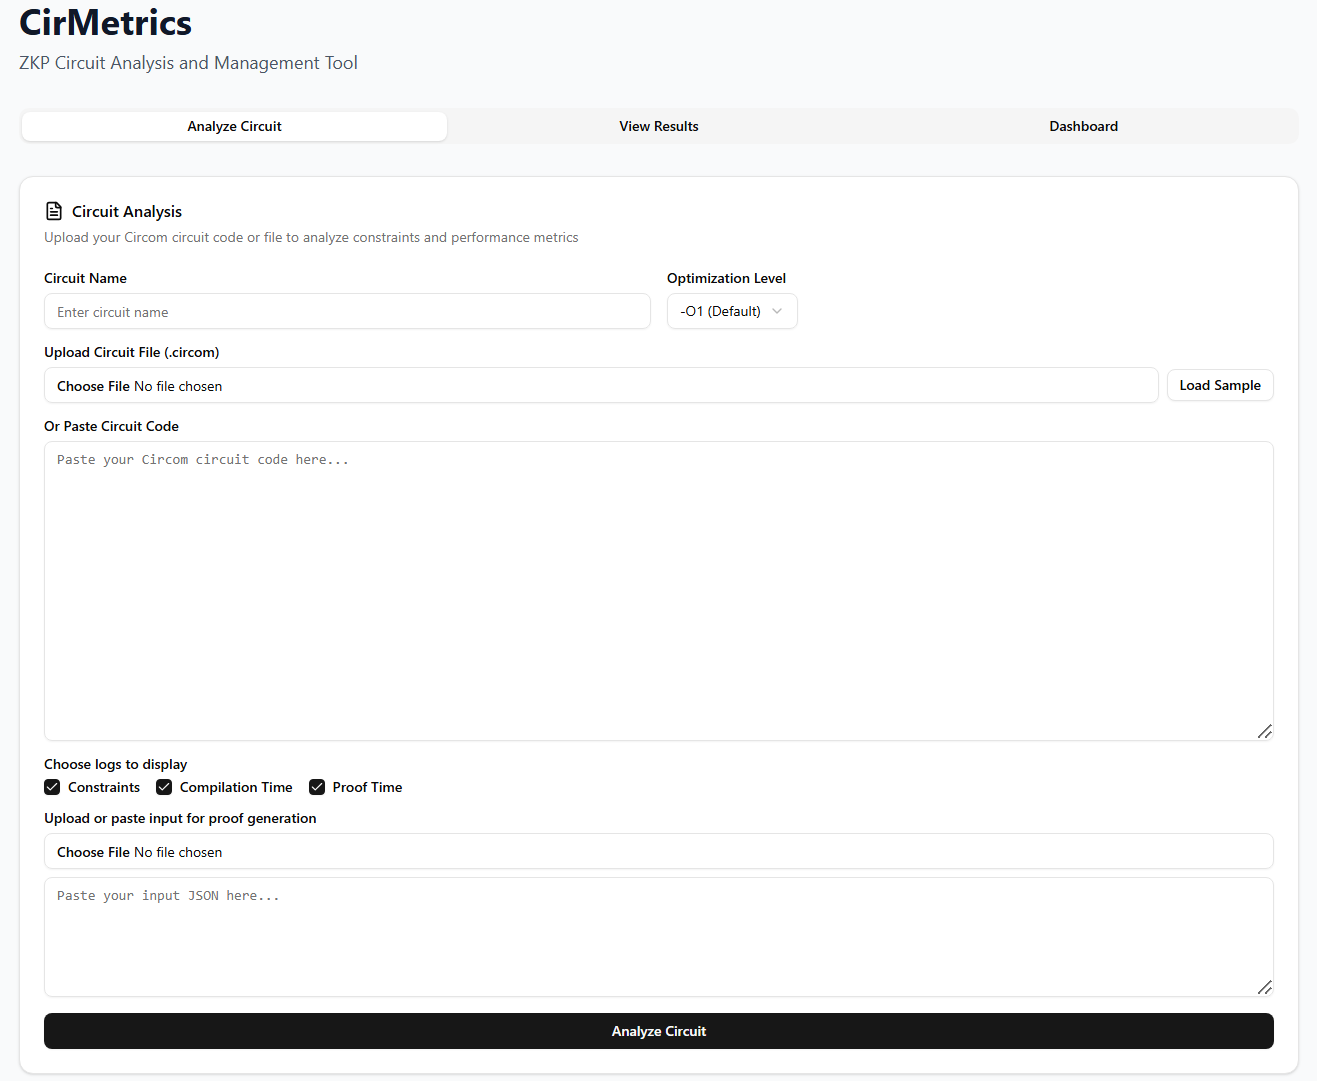
\includegraphics[width=\textwidth]{imgs/analyzescreen.png}
    \caption{Demo chức năng thực hiện phân tích mạch}
    \label{fig:chapter6-analyzescreen}
\end{figure}

Người dùng sẽ nhập tên mạch, sau đó upload file circom hoặc nhập mã nguồn mạch vào khung nhập liệu. Sau đó chọn các chức năng như "constraint" và "compilation time" để biên dịch và hiển thị các thống số của mạch. 

Người dùng cũng có thể chọn thêm "Proof Time" để tạo bằng chứng và nhập thêm đầu vào cho mạch ở dạng JSON để thực hiện tạo ZKP.

\subsection{Giao diện xem các kết quả phân tích}
\begin{figure}[H]
    \centering
    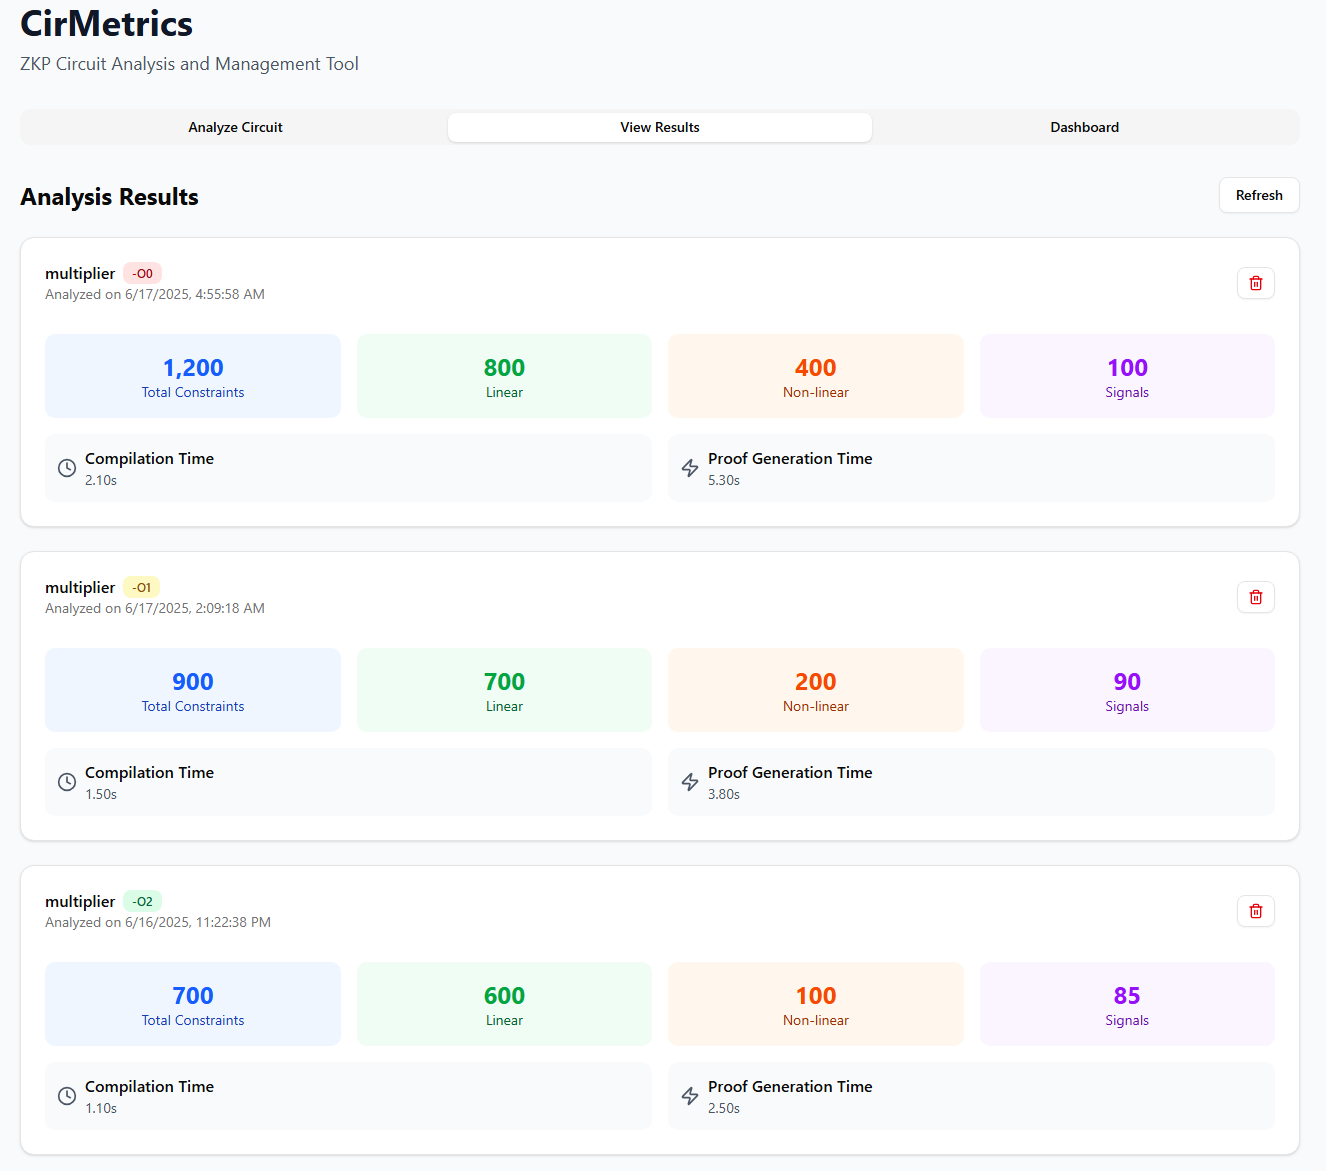
\includegraphics[width=\textwidth]{imgs/resultscreen.png}
    \caption{Demo chức năng xem các kết quả phân tích}
    \label{fig:chapter6-resultscreen}
\end{figure}

Người dung có thể xem thống số các mạch đã biên dịch và tạo bằng chứng theo thời gian. Các thông số được hiển thị bao gồm:
\begin{itemize}
    \item Thời gian biên dịch và thời gian tạo bằng chứng
    \item Số lượng ràng buộc (Tổng số lượng ràng buộc, số lượng ràng buộc tuyến tính và ràng buộc không tuyến tính).
    \item Số lượng tín hiệu của mạch.
    \item Thời gian biên dịch mạch.
    \item Thời gian tạo bằng chứng.
\end{itemize}

\subsection{Giao diện xem tổng hợp các biểu đồ về các thông số liên quan đến mạch ZK}

\begin{figure}[H]
    \centering
    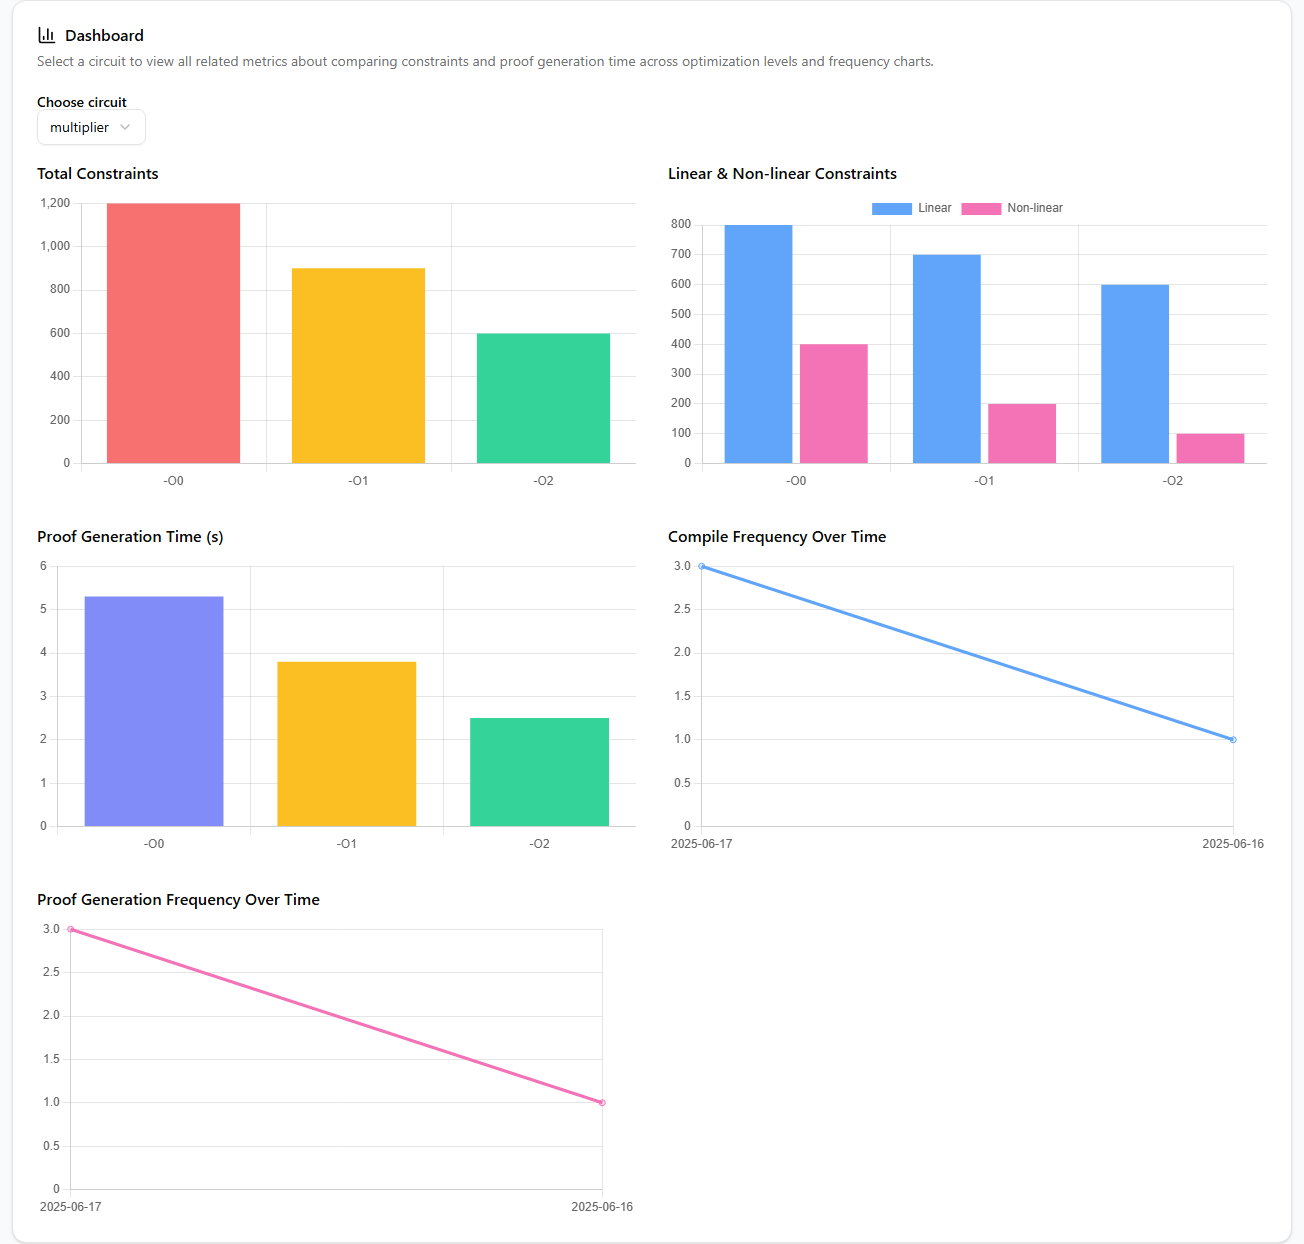
\includegraphics[width=\textwidth]{imgs/dashboardscreen.png}
    \caption{Demo chức năng xem các biểu đồ về các thông số liên quan đến mạch ZK}
    \label{fig:chapter6-dashboardscreen}
\end{figure}

Người dùng có thể chọn tên mạch và xem các biểu đồ liên quan sau:
\begin{itemize}
    \item Biểu đồ so sánh tổng lượng constraint ở các mức tối ưu mạch khác nhau.
    \item Biểu đồ so sánh tỷ lệ giữa ràng buộc tuyến tính và ràng buộc phi tuyến.
    \item Biểu đồ so sánh thời gian tạo bằng chứng ở các mức tối ưu mạch khác nhau.
    \item Biểu đồ thể hiện tần suất cập nhật mạch và tần suất tạo bằng chứng theo ngày.
\end{itemize}

Với công cụ CirMetrics, các nhà phát triển sẽ thuận tiện hơn trong việc theo dõi trực quan các thông số khi làm việc với mạch ZK. Đồng thời hỗ trợ các nhà phát triển trong việc đưa ra những quyết định hợp lí hơn khi kết hợp công cụ cùng khung \textbf{ZCLS} khi chọn phương án tối ưu hoá mạch phù hợp cho tiến trình phát triển mạch của mình.